\documentclass[12pt]{report}

%IMPORTS
\usepackage[catalan]{babel}
\usepackage[utf8]{inputenc}
\usepackage{graphicx}
\usepackage{wrapfig}
\usepackage{amsmath}
\usepackage{amssymb}
\usepackage{ragged2e} 
\usepackage{subfig}
\usepackage{caption}
\usepackage{subcaption}
\usepackage[usenames]{color}
\usepackage{xcolor}
\usepackage{float}
\usepackage{chngcntr}
\usepackage{ragged2e}
\usepackage{multirow}
\usepackage{vmargin}
\usepackage{hyperref}
\usepackage{url}

\definecolor{navy}{rgb}{0,0,128}

\setpapersize{A4}
\setmargins{2.5cm}     % margen izquierdo
{2.6cm}                % margen superior
{16.5cm}               % anchura del texto
{23.7cm}               % altura del texto
{10pt}                 % altura de los encabezados
{0cm}                  % espacio entre el texto y los encabezados
{0pt}                  % altura del pie de página
{1cm}                  % espacio entre el texto y el pie de página
\renewcommand{\baselinestretch}{1.5}

\begin{document}

\begin{titlepage}
    \centering
    {\bfseries\LARGE Universitat Autònoma de Barcelona\newline Facultat de Ciències\par}
    \vspace{2cm}
    {\hspace{-1em}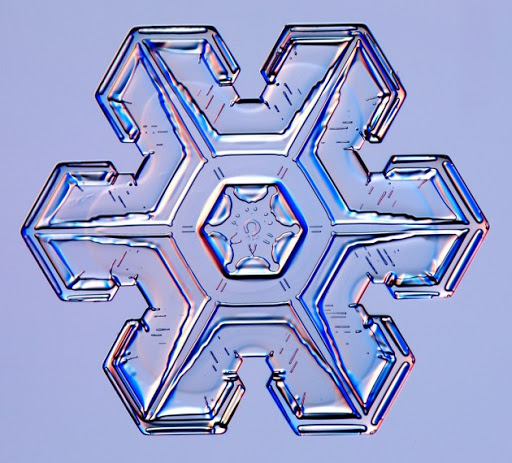
\includegraphics[width=0.4\textwidth]{flocgordi.png}\par}
    \vspace{1cm}
    {\scshape\Huge PAC 2 Probabilitat\par} %Fiat ut Nix --- et non erit nix
    \vspace{1cm}
    {\Large \itshape Autors: \par}
    {\Large Marc Bosom, Gerard Lahuerta, Ona Sánchez, Pau Ventura \par}
    \vspace{1cm}
    {\Large 11 de Juny del 2021\par}
\end{titlepage}

\justifying

\thispagestyle{empty}
\hspace{6cm}
    \begin{minipage}{0.5\linewidth}
        \vspace{10cm}%margen superior de minipage
        {\small
        % “¿Yuko, ha encontrado tu rumbo?” \\
        % El joven se arrodilló y dijo: \\
        % “Aún mejor, padre. He encontrado la nieve”.
            He aquí que mañana a estas horas yo haré llover granizo muy pesado, como nunca hubo en Egipto, desde el día que se fundó hasta ahora.
        }
        \begin{flushright}
           \citeauthor{\textit{Éxodo 9:18, Biblia}}
        \end{flushright}
        \vspace{5pt}%margen inferior de la minipage
    \end{minipage}

\newpage
\setcounter{page}{3}
\pagestyle{plain}
\tableofcontents
\cleardoublepage
\addcontentsline{}{chapter}{}

\chapter{Motivació del treball}


L'idea de fer aquest treball ve inspirada per l'hipòtesi que defensa que l'univers s'observa en un estat de no equilibri i de caos, i això permetria la formació, en qualsevol punt aleatori de l'univers i després d'una quantitat de temps molt gran, d'un cervell funcional que emuli a una persona vivint a la Terra (la qual podríem ser qualsevol de nosaltres), sense ser conscient que sigui un cervell a l'univers. \newline 
Per més informació, veure \texttt{\textcolor{navy}{\underline{\href{https://bit.ly/3fxl9hT}{aquest}}}} vídeo de \textit{QuatumFracture}.\newline
\newline El treball consisteix en una simplificació d'aquesta hipòtesi, la probabilitat que es formi un floc de neu de forma espontània. 



\chapter{Explicació de l'Experiment}

Es vol calcular la probabilitat de la formació espontània d’un floc de neu en un espai que té les característiques següents: 
\begin{itemize}
    \item Dos àtoms del mateix element tenen les mateixes qualitats físiques.
    \item Les diferents combinacions d’àtoms que donen la mateixa seqüència formen el mateix cristall.
    \item Els diferents àtoms estan distribuïts de manera aleatòria, per tant es considera simetria entre els àtoms.
\end{itemize}
Es vol crear el floc de neu a un espai que conté tres tipus diferents d’àtoms, en proporcionalitat diferent:

\begin{center}
    \begin{tabular}{c|c}
     Element & Percentatge \\ \hline
      Hidrogen (\textit{H}) & 49\%\\
      Oxigen (\textit{O}) & 49\%\\
      Buit (\textit{J}) & 2\%\\
\end{tabular}
\end{center}

En aquest espai s’hi troben un total de 100 àtoms, tots ocupen el mateix espai, estan en moviment i no hi ha mai dos àtoms en la mateixa posició. Sobre els àtoms no actua cap força externa ni interna.
\newline
El floc de neu que es vol crear és el resultat de la suma de dues molècules d’aigua ($H_2O$). Es considera que una molècula de d’aigua té l’estructura d’àtoms:
\begin{center}
    \textbf{H O H}
\end{center}
on cada lletra correspon al signe de l’àtom corresponent. Per tant, el floc de neu tindria l’estructura següent:
\begin{equation}
    \textbf{J H O H H O H J} 
    \label{eq:cristall}
\end{equation}

Els àtoms de buit (J) representen el buit, i serveixen per simular la separació de dos àtoms diferents. D’aquesta manera, només cal fixar-se en la combinació d’àtoms entre les dues J per veure si s’ha format el floc de neu.  Els àtoms sobrants dels extrems que no formin part de la formació del cristall s’anomenen impureses, i no afecten a la formació d’aquest.
\newline
A cada segon que passa, tots els àtoms de la cadena creada es reorganitzen, i d’aquesta manera la cadena va canviant. 
\\\\
Aleshores s'haurà de calcular:
\begin{enumerate}
    \item La probabilitat que es formi un floc de neu a l'espai descrit.
    \item La probabilitat que es formi un floc de neu durant una classe de probabilitat (6300 segons) mitjançant una variable aleatòria.

\end{enumerate}

\chapter{Càlculs}

\section{Definicions básiques}
L'espai on es troben els àtoms a partir dels quals es formarà el cristall s'anomena N, i la seva llargada és L (nombre d'àtoms de l'espai).\\
Es defineix \textbf{$n_{i}$} $\subset$ N com al conjunt format pels àtoms que formen el floc de neu endreçats aleatòriament de llargada $l \ ( \text{nombre d'àtoms del cristall}$). \\
L'índex $\textit{i} = \{1, 2, \cdots , L - \textit{l}\}$ \ fa referència a la posició del primer àtom del subconjunt $n$ dintre de N. \\
En aquest cas concret, es treballarà amb:
\begin{itemize}
    \item L = 100
    \item l = 8
    \item $\textit{i} = \{1, \cdots ,  92\}$ 
    \item \textbf{$n_{i}$} = conjunt d'àtoms format per  4H, 2O i 2J en qualsevol odre.
\end{itemize}


\newpage
\section{Probabilitat de la formació d'un floc de neu}

Es defineix com $P(\exists\hspace{0.25em} \text{cristall})$ com la probabilitat que existeixi un cristall al nostre espai. 
\newline Per tant, 
$$P(\exists\hspace{0.25em}\text{cristall})= P(\exists \hspace{0.25em}\text{cristall} \cap \exists\hspace{0.25em} n) =P(\exists\hspace{0.25em}\text{cristall} \hspace{0.25em} / \hspace{0.25em}\exists \hspace{0.25em}n)\cdot P(\exists \hspace{0.25em}n)$$
on en el primer igual s'ha tingut en compte que el cristall es formarà a partir d'una de les combinacions d'$n$, i en el segon s'ha aplicat la regla del producte.\\
%\ \ \ \ \forall i \in\{1,...,L-l\}=\{1,...,92\}$$ %0.001338970
S'avalua el nombre de combinacions possibles d'un grup de 8 àtoms format per 4 d'hidrogen, 2 d'oxigen i 2 de buit.
$$PR^{8}_{4,2,2}=\frac{8!}{4!\cdot2!\cdot2!}=420$$
Es calcula la probabilitat d'aconseguir la combinació \fcolorbox{red}{white}{\ref{eq:cristall}}:
$$P(\exists \hspace{0.25em} \text{cristall} \hspace{0.25em} / \hspace{0.25em} \exists \hspace{0.25em} n)=\frac{1}{PR^{8}_{4,2,2}}=\frac{1}{420}=0.00952381$$
Es calcula la probabilitat que existeixi $n$:
\begin{equation}
    P(\exists \hspace{0.25em} n)=P\left( \bigcup_{i=1}^{L-l} \exists \hspace{0.25em} n_i\right)=P\left(\bigcup_{i=1}^{92}\exists \hspace{0.25em} n_i\right)
    \label{disjuntos}
\end{equation}
Com $\{P(\exists \hspace{0.25em} n_i) : i\in\{1,2,...,92\}\}$ són disjunts dos a dos i $P(\exists \hspace{0.25em} n_1)=P(\exists \hspace{0.25em} n_2)= \hspace{-0.2em}\cdots\hspace{-0.2em}=P(\exists \hspace{0.25em} n_{92})$:
\begin{equation*}
    P(\exists \hspace{0.25em} n)=\sum_{i=1}^{92}P(\exists \hspace{0.25em} n_i)=92P(\exists \hspace{0.25em} n_q), \forall q \in \{1,2,\cdots,92\}
\end{equation*}
Es calcula la probabilitat que es formi un espai $n$; és a dir:
$$P(\exists \hspace{0.25em} n_q)=\frac{\binom{49}{4}\binom{49}{2}\binom{2}{2}}{\binom{100}{8}}=\frac{249166176}{186087894300}=0.00133897036632759 \Rightarrow$$
$$\Rightarrow P(\exists \hspace{0.25em} n)=92\cdot P(\exists \hspace{0.25em} n_q) = 92\cdot \frac{249166176}{186087894300} = \frac{5806304}{47134725}= 0.123185273702138$$

\hspace{-1.5em}Per acabar, es calcula la probabilitat que existeixi un cristall:
\begin{equation*}
    P(\exists \hspace{0.25em} \text{cristall})=P(\exists \hspace{0.25em}\text{cristall} \hspace{0.25em}/ \hspace{0.25em}\exists n)\cdot P(\exists \hspace{0.25em} n)=\frac{1}{420}\cdot \frac{5806304}{47134725} = \frac{207368}{707020875} \Rightarrow
\end{equation*}
\begin{equation}
    \Rightarrow\fcolorbox{black}{white}{$ P(\exists \hspace{0.25em}\text{cristall})=0.000293298270719376$} 
    \label{probabilitat cristall}
\end{equation}




\newpage
\section{Probabilitat que es generi un floc de neu a una classe de probabilitat}
En aquesta secció l'objectiu és calcular la probabilitat que, durant una classe de probabilitat, s'hagi format un floc de neu. Per a això es té en compte que:

\begin{enumerate}
    \item La classe dura 1 hora i 45 minuts, és a dir, 6300 segons (15 minuts per a que es ventili l'aula pel Coronavirus).
    \item Els àtoms canvien de lloc a cada segon, reorganitzant-se de forma aleatòria.
    \item Es comprova l'estat dels àtoms a cada segon.
    \item Si es troba un èxit, s'atura l'experiment.
\end{enumerate}
Així doncs, s'utilitza una variable aleatòria geomètrica, de paràmetre \textbf{p} = Probabilitat que es formi un floc de Neu \fcolorbox{red}{white}{\ref{probabilitat cristall}}.
\textbf{$$X  \thicksim G \left( p = \frac{207368}{707020875} \right)$$}
On X és la quantitat de temps que passa fins que s'aconsegueix un èxit.
\begin{equation*}
    P(X  \leqslant  6300) = \sum_{k=1}^{6300}(1-p)^{k-1}p = p\cdot \sum_{k=1}^{6300}(1-p)^{k-1}=
\end{equation*}
\begin{equation*}
    =\frac{207368}{707020875} \sum_{k=1}^{6300} \left(1-\frac{207368}{707020875} \right)^{k-1}     =0.842455943139843 \Rightarrow
\end{equation*}
\begin{equation}
     \Rightarrow\fcolorbox{black}{white}{$ P(X  \leqslant  6300)=0.842455943139843$} 
\end{equation}

\chapter{Conclusions i problemes}
Primerament, s'hagués volgut fer un cervell de Boltzman, considerant tots els àtoms de \hspace{1em} l’univers i les seves proporcions, i aquells que eren necessaris per crear un cervell, amb el seu ordre corresponent. A l'hora de fer els càlculs, els valors de les dimensions eren massa elevats, com en el cas de $\#\Omega = 10^{84}!$, la qual indica les diferents combinacions que es poden fer considerant tots els àtoms de l'univers. Es va intentar calcular a partir de la fòrmula de Stirling i la funció Gamma, però el temps de càlcul per a fer totes les operacions superava el temps de vida del Sistema Solar, de manera que es va decidir fer la simplificació que s'ha vist en el treball.\newline


A l’hora de fer els càlculs en R, com que es treballava amb probabilitats molt petites, va sorgir la necessitat d'optimitzar el programa el màxim possible perquè funcionés més ràpidament. 
A més, com que les probabilitats eren de l'ordre de $10^{-3}$, calien moltes repeticions per poder determinar amb precisió la probabilitat.  Es van repetir les simulacions en 4 ordinadors simultàniament, i en cadascun d'ells es van fer un total de 5.000.000 repeticions.
La probabilitat teòrica de l'experiment, calculada a partir d'un \textit{script} de \textit{SageMath} és:
\begin{equation*}
0.000293298270719376
\end{equation*}
\newpage
I la mitjana de les probabilitats obtingudues a partir de les simulacions en R va ser:

\begin{center}
    \begin{tabular}{cc|c}
     Simulació & Resultat & Mitjana \\ \hline
      1 & 0.0003008\\
      2 & 0.0002926\\
      3 & 0.0002900 & 0.00029576\\
      4 & 0.0002982\\
      5 & 0.0002972\\
\end{tabular}
\end{center}

Respecte al moviment entre els àtoms, al principi es va plantejar de manera que, a cada instant de temps, dos àtoms intercanviessin la seva posició, fent servir una variable aleatòria exponencial. Però degut a problemes amb l'\textit{stript} de R es va decidir que els instants de temps fossin discrets, és a dir, que en cada instant de temps canviés la distribució de tots els àtoms aleatòriament, com en una geomètrica.\newline

En el càlcul de la probabilitat de l'existència d'un cristall, van sorgir diferents dificultats, perquè el nombre d'interseccions que hi havia conduïen a càlculs complexos i llargs. Per això, es va plantejar el problema de forma disjunta \fcolorbox{red}{white}{\ref{disjuntos}}: va formular-se de tal manera que el cristall contingués tots els àtoms de buit que hi havia a l'espai (els 2 àtoms de buit de l'espai es troben al principi i final de la cadena del cristall \fcolorbox{red}{white}{\ref{eq:cristall}}), per convertir els elements en disjunts, ja que, si tots els àtoms d’aquell element estaven en un interval, no podien estar a cap altre.
\newpage
\textcolor{white}{easter egg}
\end{document}
